\documentclass{article}
\usepackage[margin=0.75in]{geometry}
\usepackage{tikz}
\usetikzlibrary{positioning,arrows.meta,calc,fit,backgrounds}
\usepackage{tcolorbox}
\usepackage{xcolor}
\usepackage{skak}

\newcommand{\benchmark}{ChessChain}

\begin{document}

\begin{figure}[t]
    \centering

    % Chess problem - Version 6: Better whitespace utilization
    \begin{tcolorbox}[
        title=\textbf{Chess: Minimax Search} \hfill {\small\colorbox{orange!20}{Easy} \quad 6 orderings},
        colframe=orange!70!black,
        colback=orange!3,
        boxrule=0.8pt,
        width=\textwidth
    ]
    \small

    \begin{minipage}[c]{0.22\textwidth}
        \centering
        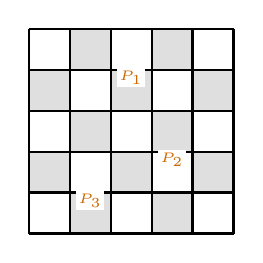
\begin{tikzpicture}[scale=0.52]
            % Draw 5x5 board
            \foreach \x in {0,...,4} {
                \foreach \y in {0,...,4} {
                    \pgfmathparse{mod(\x+\y,2) ? "gray!25" : "white"}
                    \fill[\pgfmathresult] (\x,\y) rectangle (\x+1,\y+1);
                }
            }
            \draw[thick] (0,0) grid (5,5);
            % Knight at (0,4)
            \node at (0.5,4.5) {\small$\symknight$};
            % Pawns with labels
            \node at (2.5,4.5) {\small$\sympawn$};
            \node[font=\tiny, orange!80!black, fill=white, inner sep=1pt] at (2.5,3.8) {$P_1$};
            \node at (3.5,2.5) {\small$\sympawn$};
            \node[font=\tiny, orange!80!black, fill=white, inner sep=1pt] at (3.5,1.8) {$P_2$};
            \node at (1.5,1.5) {\small$\sympawn$};
            \node[font=\tiny, orange!80!black, fill=white, inner sep=1pt] at (1.5,0.8) {$P_3$};
        \end{tikzpicture}

        \vspace{0.1cm}
        {\scriptsize Knight captures}\\[-0.05cm]
        {\scriptsize all three pawns}
    \end{minipage}%
    \hfill%
    \begin{minipage}[c]{0.76\textwidth}
        \centering
        \begin{tikzpicture}[
            node distance=0.4cm and 0.6cm,
            every node/.style={font=\scriptsize},
            bfsbox/.style={draw, rounded corners=3pt, fill=orange!10, thick, draw=orange!40, inner sep=3pt, align=center},
            treegroup/.style={draw, rounded corners=3pt, fill=orange!22, thick, draw=orange!50, inner sep=4pt, align=center},
            outputnode/.style={draw, rounded corners=3pt, fill=orange!45, minimum width=1.0cm, minimum height=0.5cm, thick, draw=orange!70, font=\scriptsize\bfseries},
            arrow/.style={-{Stealth[length=2mm]}, thick, orange!55!black}
        ]
            % BFS box (left)
            \node[bfsbox] (bfs) {
                \textbf{BFS distances}\\[1pt]
                {\footnotesize $d_{K,P_1}, d_{K,P_2}, d_{K,P_3}$}\\[0pt]
                {\footnotesize $d_{P_1,P_2}, d_{P_1,P_3}, d_{P_2,P_3}$}
            };

            % Game tree box (right of BFS)
            \node[treegroup, right=0.8cm of bfs] (tree) {
                \textbf{Minimax tree}\\[2pt]
                \begin{tikzpicture}[
                    scale=0.85,
                    every node/.style={font=\tiny},
                    maxn/.style={draw, circle, fill=orange!12, minimum size=0.38cm, inner sep=0pt, thick, draw=orange!45},
                    minn/.style={draw, rectangle, fill=orange!38, minimum size=0.32cm, inner sep=1pt, thick, draw=orange!60},
                    leafn/.style={draw, circle, fill=orange!55, minimum size=0.22cm, inner sep=0pt, thick, draw=orange!70}
                ]
                    % Root
                    \node[maxn] (r) {};
                    \node[font=\tiny, anchor=west] at (r.east) {\,MAX};

                    % Level 1 - MIN nodes
                    \node[minn, below left=0.32cm and 0.55cm of r] (a1) {\tiny$P_1$};
                    \node[minn, below=0.35cm of r] (a2) {\tiny$P_2$};
                    \node[minn, below right=0.32cm and 0.55cm of r] (a3) {\tiny$P_3$};
                    \node[font=\tiny, anchor=west] at (a3.east) {\,MIN};

                    % Leaves
                    \node[leafn, below left=0.28cm and 0.12cm of a1] (l1) {};
                    \node[leafn, below right=0.28cm and 0.12cm of a1] (l2) {};
                    \node[leafn, below left=0.28cm and 0.12cm of a2] (l3) {};
                    \node[leafn, below right=0.28cm and 0.12cm of a2] (l4) {};
                    \node[leafn, below left=0.28cm and 0.12cm of a3] (l5) {};
                    \node[leafn, below right=0.28cm and 0.12cm of a3] (l6) {};

                    % Edges
                    \draw[semithick, orange!35] (r) -- (a1);
                    \draw[semithick, orange!35] (r) -- (a2);
                    \draw[semithick, orange!35] (r) -- (a3);
                    \draw[thin, orange!35] (a1) -- (l1);
                    \draw[thin, orange!35] (a1) -- (l2);
                    \draw[thin, orange!35] (a2) -- (l3);
                    \draw[thin, orange!35] (a2) -- (l4);
                    \draw[thin, orange!35] (a3) -- (l5);
                    \draw[thin, orange!35] (a3) -- (l6);

                    % Label
                    \node[font=\tiny, orange!60!black] at ([yshift=-0.08cm]$(l3)!0.5!(l4)$) {$3!=6$};
                \end{tikzpicture}
            };

            % Output (below and between)
            \node[outputnode, below=0.5cm of $(bfs.south)!0.5!(tree.south)$] (out) {\textbf{Output}};

            % Arrows
            \draw[arrow] (bfs.east) -- (tree.west);
            \draw[arrow] (tree.south) -- (out.north);

        \end{tikzpicture}
    \end{minipage}

    \vspace{0.05cm}
    \hrule
    \vspace{0.08cm}

    {\footnotesize
    \textit{Step 1:} BFS computes shortest knight paths between all position pairs.
    \textit{Step 2:} Minimax evaluates $3!$ capture orderings (Alice maximizes, Bob minimizes).
    }

    \vspace{0.1cm}
    \hfill \textbf{Answer:} [Redacted]
    \end{tcolorbox}

    \caption{\textbf{Chess:} \colorbox{orange!10}{BFS} $\to$ \colorbox{orange!22}{Minimax tree} $\to$ \colorbox{orange!45}{Output}. Circle = MAX (Alice), square = MIN (Bob).}
\end{figure}

\end{document}
